\documentclass[11pt,spanish]{article}

\usepackage{listings}             
\usepackage{anysize} 
\usepackage{graphicx}
\usepackage[spanish]{babel}
\usepackage[utf8]{inputenc}
\usepackage{xcolor}
\usepackage{wrapfig}
\usepackage{amsmath}


\renewcommand\lstlistingname{Código}
\lstset{language=Python}
\marginsize{1cm}{1cm}{2cm}{2cm}
\selectlanguage{spanish}
\lstset{
language=Python,
 backgroundcolor=\color{red!75!green!50!blue!25},
 frame=single,
literate=
  {á}{{\'a}}1 {é}{{\'e}}1 {í}{{\'i}}1 {ó}{{\'o}}1 {ú}{{\'u}}1
  {Á}{{\'A}}1 {É}{{\'E}}1 {Í}{{\'I}}1 {Ó}{{\'O}}1 {Ú}{{\'U}}1
  {à}{{\`a}}1 {è}{{\`e}}1 {ì}{{\`i}}1 {ò}{{\`o}}1 {ù}{{\`u}}1
  {À}{{\`A}}1 {È}{{\'E}}1 {Ì}{{\`I}}1 {Ò}{{\`O}}1 {Ù}{{\`U}}1
  {ä}{{\"a}}1 {ë}{{\"e}}1 {ï}{{\"i}}1 {ö}{{\"o}}1 {ü}{{\"u}}1
  {Ä}{{\"A}}1 {Ë}{{\"E}}1 {Ï}{{\"I}}1 {Ö}{{\"O}}1 {Ü}{{\"U}}1
  {â}{{\^a}}1 {ê}{{\^e}}1 {î}{{\^i}}1 {ô}{{\^o}}1 {û}{{\^u}}1
  {Â}{{\^A}}1 {Ê}{{\^E}}1 {Î}{{\^I}}1 {Ô}{{\^O}}1 {Û}{{\^U}}1
  {œ}{{\oe}}1 {Œ}{{\OE}}1 {æ}{{\ae}}1 {Æ}{{\AE}}1 {ß}{{\ss}}1
  {ű}{{\H{u}}}1 {Ű}{{\H{U}}}1 {ő}{{\H{o}}}1 {Ő}{{\H{O}}}1
  {ç}{{\c c}}1 {Ç}{{\c C}}1 {ø}{{\o}}1 {å}{{\r a}}1 {Å}{{\r A}}1
  {€}{{\EUR}}1 {£}{{\pounds}}1
}


\title{\vspace{-3cm} \textbf{\huge Universidad de Sonora} \\ \LARGE Actividad 11: \textbf{Apocalipsis Zombie }}
\author{\textsc{Andrés Ignacio Rodríguez Mendoza}}
\date{}

\begin{document}

\begin{wrapfigure}{r}{0.2\textwidth}
  \begin{center}
   \vspace{-5.8cm} 
\includegraphics[width=0.15\textwidth]{uni}
  \end{center}
\end{wrapfigure}

\maketitle  
\begin{center}
\rule{\textwidth}{1pt}
\end{center}

Se implementan modelos para simular la evolución de sistemas biológicos en función del tiempo sometidos a parámetros de conversión entre clases. Cada elemento del sistema pertenece a una clase. Se impone la conservación (en un periodo corto de tiempo) del número de individuos para mantener congruencia en el sistema; ésto es, así como sale un elemento de una clase entra en otra, dado que los modelos sólo mudan elementos de una clase a otra.
Se realizan varios modelos variando la cantidad de clases y las interacciones entre ellas.\\

\textbf{Modelo Básico}\\
Las clases son:
\begin{itemize}
\item Susceptible $(S)$
\item Zombie $(Z)$
\item Removido $(R)$
\end{itemize}
Los parámetros:
\begin{itemize}
\item Elementos de $S$ mudan a $R$ a razón del parámetro $\delta$.
\item Elementos de $R$ mudan a $Z$ a razón de $\zeta$.
\item Elementos de $S$ mudan a $Z$ a razón de $\beta$.
\item Elementos de $Z$ mudan a $R$ a razón de $\alpha$.
\item La taza de nacimiento $\Pi$ puede despreciarse en un periodo corto de tiempo.
\end{itemize}
Las ecuaciónes que gobiernan el modelo:
\begin{align*}
S' \ & = \ \Pi - \beta S Z - \delta S\\
Z' \ & = \ \beta S Z + \zeta R - \alpha S Z\\
R' \ & = \ \delta S + \alpha S Z - \zeta R.
\end{align*}

\textbf{Modelo con Infección Latente}\\
En el \textit{Modelo Básico} se introduce una nueva clase de individuos, y se modifican las relaciones entre elementos de clases. Las clases son:
\begin{itemize}
\item Susceptible $(S)$
\item Infectado $(I)$
\item Zombie $(Z)$
\item Removido $(R)$
\end{itemize}
Los parámetros:
\begin{itemize}
\item Elementos de $S$ mudan a $R$ a razón de $\delta$.
\item Elementos de $I$ mudan a $R$ a razón de $\delta$.
\item Elementos de $I$ mudan a $Z$ a razón de $\rho$.
\item Elementos de $R$ mudan a $Z$ a razón de $\zeta$.
\item Elementos de $S$ mudan a $I$ a razón de $\beta$.
\item Elementos de $Z$ mudan a $R$ a razón de $\alpha$.
\end{itemize}
Las ecuaciónes que gobiernan el modelo:
\begin{align*}
S' \ & = \ \Pi - \beta S Z - \delta S\\
I' \ & = \ \beta S Z - \rho I - \delta I\\
Z' \ & = \ \rho I + \zeta R - \alpha S Z\\
R' \ & = \ \delta S + \delta I + \alpha S Z - \zeta R.
\end{align*}

\textbf{Modelo con Cuarentena}\\
En el \textit{Modelo con Infección Latente} se introduce otra clase y se afectan las transiciones. La clase que se agrega es:
\begin{itemize}
\item Cuarentena $(Q)$
\end{itemize}
Y las transiciones correspondientes a esta clase:
\begin{itemize}
\item Elementos de $I$ mudan a $Q$ a razón de $\kappa$.
\item Elementos de $Z$ mudan a $Q$ a razón de $\sigma$.
\item Elementos de $Q$ mudan a $R$ a razón de $\gamma$.
\end{itemize}
Se adieren estas transiciones a las ecuaciones del modelo y una nueva ecuación correspondiente a $Q$:
\begin{align*}
S' \ & = \ \Pi - \beta S Z - \delta S\\
I' \ & = \ \beta S Z - \rho I - \delta I - \kappa I\\
Z' \ & = \ \rho I + \zeta R - \alpha S Z - \sigma Z\\
R' \ & = \ \delta S + \delta I + \alpha S Z - \zeta R + \gamma Q\\
Q' \ & = \ \kappa I + \kappa Z - \gamma Q.
\end{align*}

\textbf{Modelo con Tratamiento}\\
Al \textit{Modelo con Infección Latente} se añade un nuevo factor que permite mover elementos de $Z$ a $S$. La nueva transición de elemento es:
\begin{itemize}
\item Elementos de $Z$ mudan a $S$ a razón de $c$.
\end{itemize}
Las ecuaciones quedan:
\begin{align*}
S' \ & = \ \Pi - \beta S Z - \delta S + c Z \\
I' \ & = \ \beta S Z - \rho I - \delta I \\
Z' \ & = \ \rho I + \zeta R - \alpha S Z - c Z\\
R' \ & = \ \delta S + \delta I + \alpha S Z - \zeta R.
\end{align*}

\textbf{Erradicación Impulsiva}\\
El \textit{Modelo básico} lo integramos en intervalos periódicos. Entre cada intervalo se elimina cierto porcentaje de elementos de $Z$ hasta que $Z=0$. Las ecuaciones quedan: 
\begin{align*}
S' \ & = \ \Pi - \beta S Z - \delta S &t \neq t_n \\
Z' \ & = \ \beta S Z + \zeta R - \alpha S Z	& t \neq t_n \\
R' \ & = \ \delta S + \alpha S Z - \zeta R	& t \neq t_n  \\
Z  \ & = \ -k n Z  \	& t = t_n,  
\end{align*}
donde $ k \in [0,1)$ es la taza de eliminación y $n$ el número de intervalos requeridos para $ k n \geq 1$. 


\section*{Código}

\begin{lstlisting}

# zombie apocalypse modeling
import numpy as np
import matplotlib.pyplot as plt
from scipy.integrate import odeint
plt.ion()
plt.rcParams['figure.figsize'] = 10, 8


P = 0       # birth rate
d = 0.0000  # natural death percent (per day)
B = 0.0095  # transmission percent  (per day)
G = 0.0001  # resurect percent (per day)
A = 0.0001  # destroy percent  (per day)
r = 0.5000  # infection rate 
k = 0.0220  # infected on quarentine rate
s = 0.0220  # zombies on quarentine rate
e = 0.0010  # killed because escaping
c = 0.200  # cure effectiveness rate


# Los modelos 
def Basic(y, t):
	Si = y[0]
	Ii = y[1]
	Zi = y[2]
	Ri = y[3]	
	f0 = P - B*Si*Zi - d*Si
	f1 = B*Si*Zi + G*Ri - A*Si*Zi
	f2 = d*Si + A*Si*Zi - G*Ri
	return [f0, f2, f1, 0, 0]

def LatentInfection(y, t):
	Si = y[0]
	Ii = y[1]
	Zi = y[2]
	Ri = y[3]
	f0 = P - B*Si*Zi - d*Si
	f1 = B*Si*Zi - r*Ii - d*Ii
	f2 = r*Ii + G*Ri - A*Si*Zi
	f3 = d*Si + d*Ii + A*Si*Zi - G*Ri
	return [f0, f1, f2, f3, 0]


def Quarantine(y,t):
	Si = y[0]
	Ii = y[1]
	Zi = y[2]
	Ri = y[3]
	Qi = y[4]	
	f0 = P - B*Si*Zi - d*Si
	f1 = B*Si*Zi - r*Ii - d*Ii - k*Ii
	f2 = r*Ii + G*Ri - A*Si*Zi - s*Zi
	f3 = d*Si + d*Ii + A*Si*Zi - G*Ri + e*Qi
	f4 = k*Ii + s*Zi - e*Qi	
	return [f0, f1, f2, f3, f4]
	
def Treatment(y,t):
    Si = y[0]
    Ii = y[1]
    Zi = y[2]
    Ri = y[3]
    f0 = P - B*Si*Zi - d*Si + c*Zi
    f1 = B*Si*Zi - r*Ii - d*Ii
    f2 = r*Ii + G*Ri - A*Si*Zi - c*Zi
    f3 = d*Si + d*Ii + A*Si*Zi - G*Ri
    return [f0, f1, f2, f3, 0]



# initial conditions
S0 = 500.                   # initial population
I0 = 0                      # initial infected people
Z0 = 0                      # initial zombie population
R0 = 0                      # initial death population
Q0 = 0                      # initial quarantine population

y0 = [S0, I0, Z0, R0, Q0]   # initial condition vector

t  = np.linspace(0, 20., 1000)       # time grid

# solve the DEs and plot
soln = odeint(Basic, y0, t)
S = soln[:, 0]
R = soln[:, 1]
Z = soln[:, 2]
I = soln[:, 3]
Q = soln[:, 4]
plt.plot(t, S, label='Living')
plt.plot(t, Z, label='Zombies')
plt.xlabel('Days from outbreak')
plt.ylabel('Population')
plt.ylim(-1,501)
plt.title('Zombie Apocalypse - Basic Model Zero Zombies')
plt.show()

# we change the parameters and initial zombies
Z0 = 2
A  = 0.005
y0 = [S0, I0, Z0, R0, Q0]

soln = odeint(Basic, y0, t)
S = soln[:, 0]
R = soln[:, 1]
Z = soln[:, 2]
I = soln[:, 3]
Q = soln[:, 4]
plt.plot(t, S, label='Living')
plt.plot(t, Z, label='Zombies')
plt.xlabel('Days from outbreak')
plt.ylabel('Population')
plt.title('Zombie Apocalypse - Basic Model')
plt.show()

soln = odeint(LatentInfection, y0, t)
S = soln[:, 0]
I = soln[:, 1]
Z = soln[:, 2]
R = soln[:, 3]
Q = soln[:, 4]
plt.plot(t, S, label='Living')
plt.plot(t, Z, label='Zombies')
plt.xlabel('Days from outbreak')
plt.ylabel('Population')
plt.title('Zombie Apocalypse - Latent Infection')
plt.show()

soln = odeint(Quarantine, y0, t)
S = soln[:, 0]
I = soln[:, 1]
Z = soln[:, 2]
R = soln[:, 3]
Q = soln[:, 4]
plt.plot(t, S, label='Living')
plt.plot(t, Z, label='Zombies')
plt.xlabel('Days from outbreak')
plt.ylabel('Population')
plt.title('Zombie Apocalypse - Quarantine')
plt.show()

soln = odeint(Treatment, y0, t)
S = soln[:, 0]
I = soln[:, 1]
Z = soln[:, 2]
R = soln[:, 3]
Q = soln[:, 4]
plt.title('Zombie Apocalypse')
plt.plot(t, S, label='Living')
plt.plot(t, Z, label='Zombies')
plt.xlabel('Days from outbreak')
plt.ylabel('Population')
plt.title('Zombie Apocalypse - Treatment')
plt.show()


# Eradication with impulsive attacks each 2.5 days
A = 0.00545; B = 0.0075; G = 0.09; d = 0.0001
t1  = np.linspace(0, 2.5, 300)
t2  = np.linspace(2.5, 5., 300)
t3  = np.linspace(5, 7.5, 300)
t4  = np.linspace(7.5, 10.,300)

soln = odeint(Basic, y0, t1)
S = soln[:, 0]
Z = soln[:, 2]
sol1 = odeint(Basic,[soln[299, 0],soln[299, 1],0.75*soln[299, 2],0,0], t2)
S = np.concatenate((S,sol1[:, 0]))
Z = np.concatenate((Z,sol1[:, 2]))
sol2 = odeint(Basic,[sol1[299, 0],sol1[299, 1],0.50*sol1[299, 2],0,0], t3)
S = np.concatenate((S,sol2[:, 0]))
Z = np.concatenate((Z,sol2[:, 2]))
sol3 = odeint(Basic,[sol2[299, 0],sol2[299, 1],0.25*sol2[299, 2],0,0], t4)
S = np.concatenate((S,sol3[:, 0]))
Z = np.concatenate((Z,sol3[:, 2]))


t = np.concatenate((t1,t2,t3,t4))

plt.plot(t, Z, color= 'g' , label='Zombies')
plt.xlabel('Days from outbreak')
plt.ylabel('Zombies')
plt.title('Zombie Apocalypse - Eradication')
plt.show()
\end{lstlisting}


\section*{Gáficas}

\centering

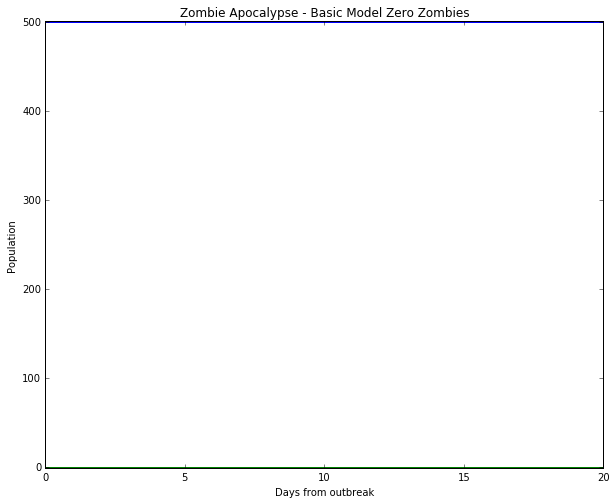
\includegraphics[scale=0.8]{0}\\
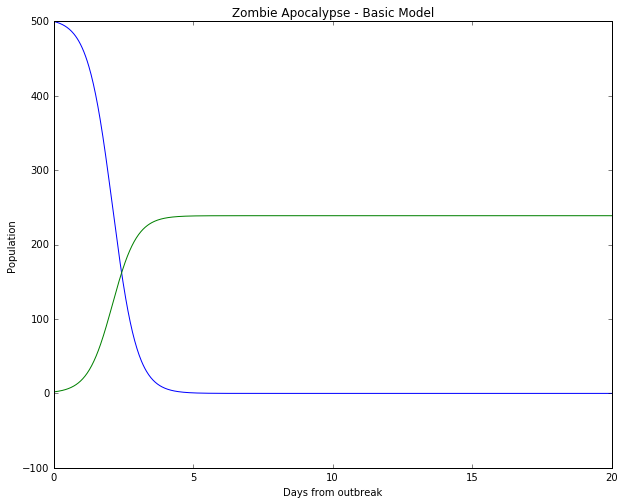
\includegraphics[scale=0.8]{basic}\\
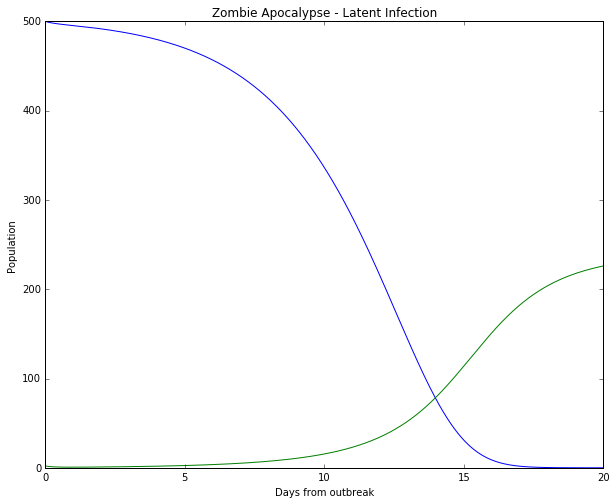
\includegraphics[scale=0.8]{lat}\\
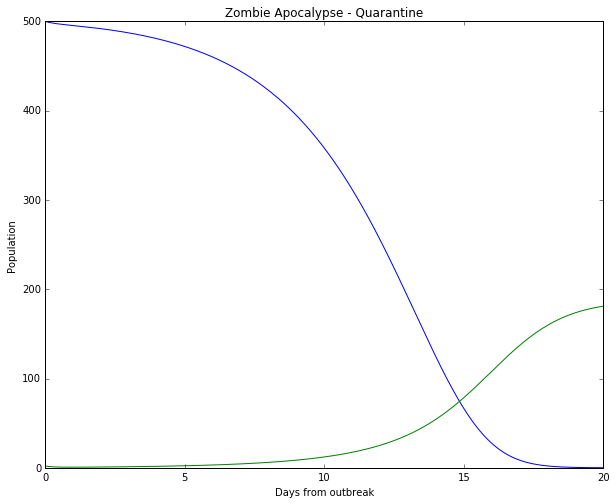
\includegraphics[scale=0.8]{q}\\
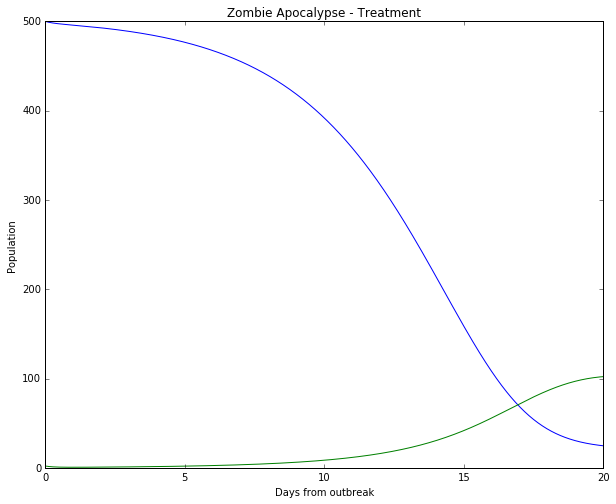
\includegraphics[scale=0.8]{cure}\\
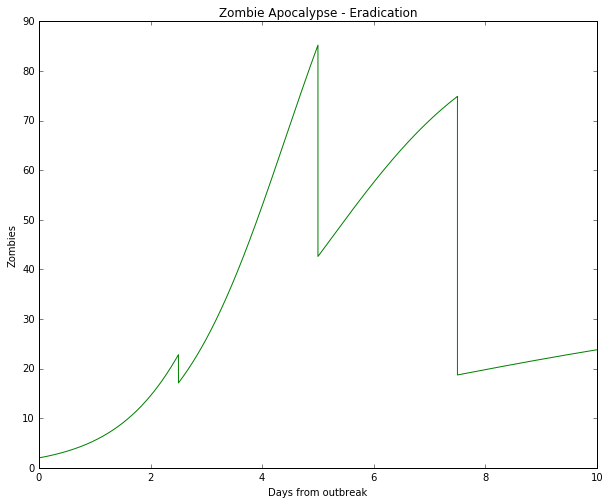
\includegraphics[scale=0.8]{er}\\





\end{document}
